% LaTeX document that includes all possible types of CC-licensed images
% "CC-*:" tokens and their values are the annotations that the compliance
% checking tool uses:
% CC-Lic: BY
% CC-Attribution-Name: Matthew Bohnsack
% CC-Attribution-URL: http://bohnsack.com/
% CC-Commercial-Use: T
\documentclass[mathserif,xcolor=dvipsnames,hyperref={bookmarks=true}]{beamer}
\usepackage{eulervm}
\usepackage{courier}
\usepackage{listings}
\usefonttheme{structurebold}
\usecolortheme[named=Maroon]{structure}
\usetheme{Antibes}
\usecolortheme{lily}
\useoutertheme{infolines}
\setbeamertemplate{navigation symbols}{}

\newcommand{\mytitle}{Test Document 01}
\newcommand{\myauthor}{Matthew Paul Bohnsack}

\title{Test Document 01}
\author[Matthew Bohnsack]{Matthew Paul Bohnsack}
\institute[UNM]{University of New Mexico\\Albuquerque, New Mexico USA}

\begin{document}

\begin{frame}
    \titlepage
\end{frame}

\section{Introduction}

\subsection{Some Images}

%%%%%%%%% My images %%%%%%%%%%%%%%%%%%%%%%%%%%%%%%%%%%%%%%%%%%%%%%%
\begin{frame}[t]
    \frametitle{My image under CC0}
    \begin{center}
        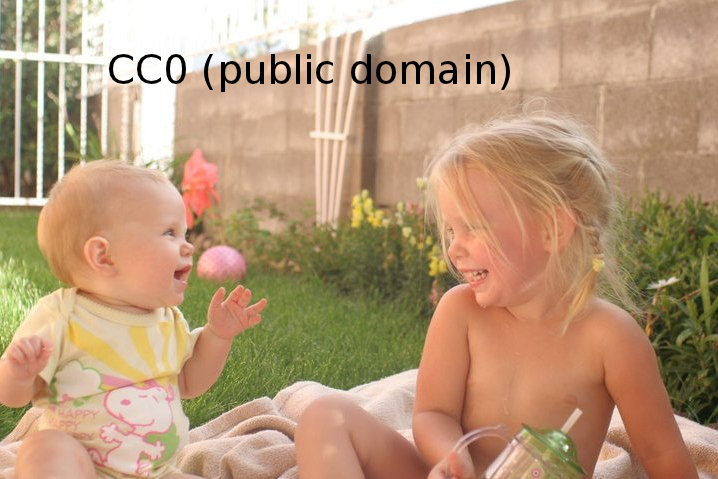
\includegraphics[width=0.8\textwidth]{../images/mine/cc0.jpg}
    \end{center}
\end{frame}
\begin{frame}[t]
    \frametitle{My image under CC BY}
    \begin{center}
        
\includegraphics[width=0.8\textwidth]{../images/mine/cc-by.jpg}
    \end{center}
\end{frame}
\begin{frame}[t]
    \frametitle{My image under CC BY-SA}
    \begin{center}
        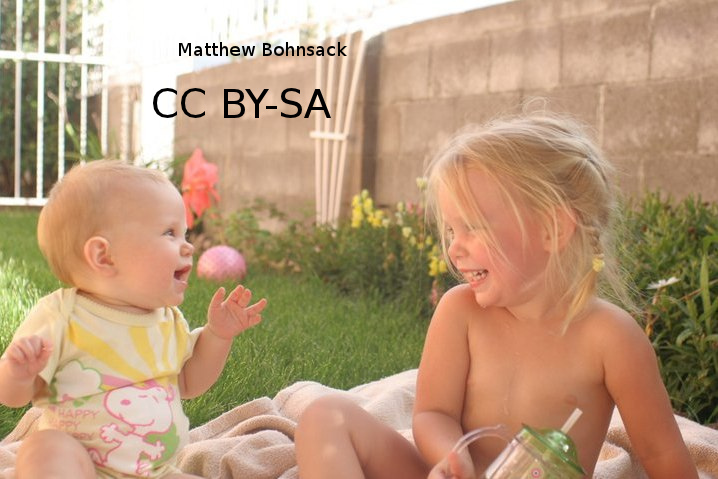
\includegraphics[width=0.8\textwidth]{../images/mine/cc-by-sa.jpg}
    \end{center}
\end{frame}
\begin{frame}[t]
    \frametitle{My image under CC BY-ND}
    \begin{center}
        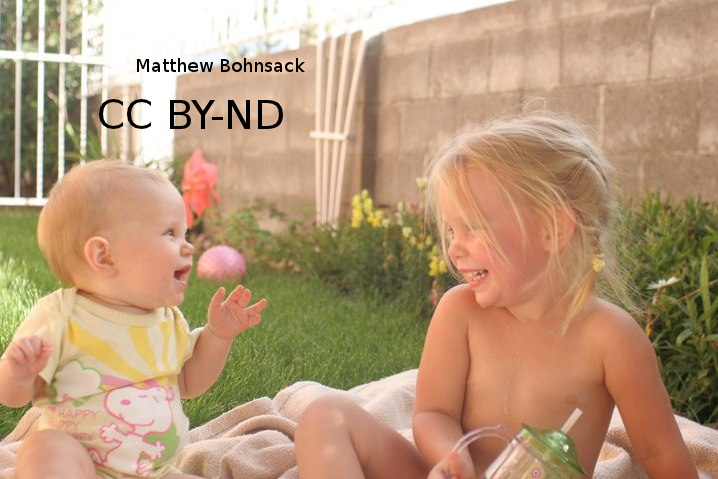
\includegraphics[width=0.8\textwidth]{../images/mine/cc-by-nd.jpg}
    \end{center}
\end{frame}
\begin{frame}[t]
    \frametitle{My image under CC BY-NC}
    \begin{center}
        
\includegraphics[width=0.8\textwidth]{../images/mine/cc-by-nc.jpg}
    \end{center}
\end{frame}
\begin{frame}[t]
    \frametitle{My image under CC BY-NC-SA}
    \begin{center}
        
\includegraphics[width=0.8\textwidth]{../images/mine/cc-by-nc-sa.jpg}
    \end{center}
\end{frame}
\begin{frame}[t]
    \frametitle{My image under CC BY-NC-ND}
    \begin{center}
        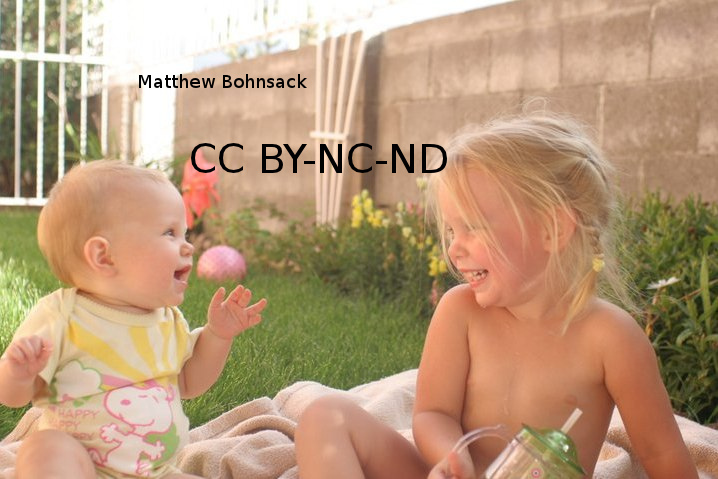
\includegraphics[width=0.8\textwidth]{../images/mine/cc-by-nc-nd.jpg}
    \end{center}
\end{frame}

%%%%%%%%% Someone else's images %%%%%%%%%%%%%%%%%%%%%%%%%%%%%%%%%%%%%%%%%%%%%%%
\begin{frame}[t]
    \frametitle{Someone else's image under CC BY}
    \begin{center}
        
\includegraphics[width=0.8\textwidth]{../images/others/cc-by.jpg}
    \end{center}
\end{frame}
\begin{frame}[t]
    \frametitle{Someone else's image under CC BY-SA}
    \begin{center}
        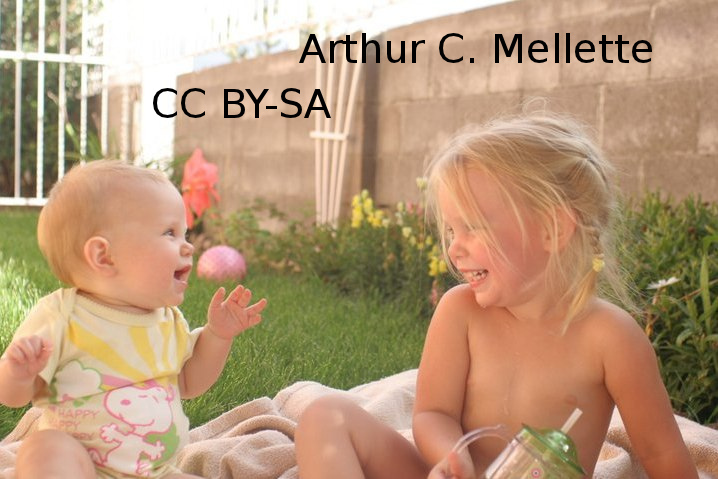
\includegraphics[width=0.8\textwidth]{../images/others/cc-by-sa.jpg}
    \end{center}
\end{frame}
\begin{frame}[t]
    \frametitle{Someone else's image under CC BY-ND}
    \begin{center}
        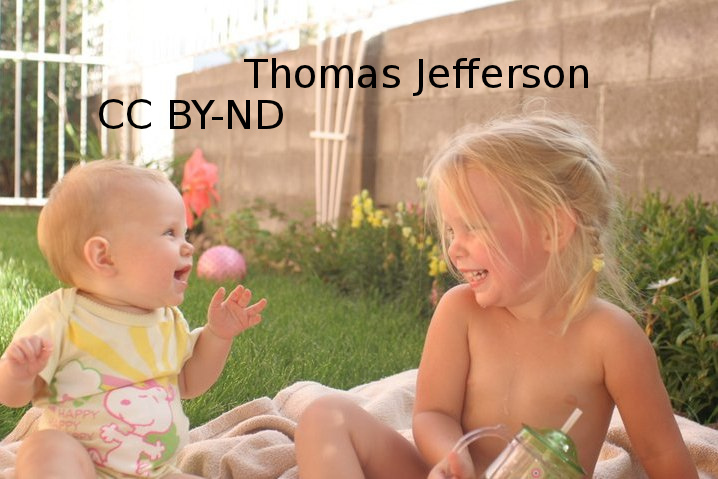
\includegraphics[width=0.8\textwidth]{../images/others/cc-by-nd.jpg}
    \end{center}
\end{frame}
\begin{frame}[t]
    \frametitle{Someone else's image under CC BY-NC}
    \begin{center}
        
\includegraphics[width=0.8\textwidth]{../images/others/cc-by-nc.jpg}
    \end{center}
\end{frame}
\begin{frame}[t]
    \frametitle{Someone else's image under CC BY-NC-SA}
    \begin{center}
        
\includegraphics[width=0.8\textwidth]{../images/others/cc-by-nc-sa.jpg}
    \end{center}
\end{frame}
\begin{frame}[t]
    \frametitle{Someone else's image under CC BY-NC-ND}
    \begin{center}
        
\includegraphics[width=0.8\textwidth]{../images/others/cc-by-nc-nd.jpg}
    \end{center}
\end{frame}

\end{document}
